\documentclass[letterpaper]{article}
\usepackage[margin=1in]{geometry}
\usepackage[utf8]{inputenc}
\usepackage{textcomp}
\usepackage{amssymb}
\usepackage{natbib}
\usepackage{graphicx}
\usepackage{gensymb}
\usepackage{amsthm, amsmath, mathtools}
\usepackage[dvipsnames]{xcolor}
\usepackage{enumerate}
\usepackage{mdframed}
\usepackage[most]{tcolorbox}
\usepackage{csquotes}
% https://tex.stackexchange.com/questions/13506/how-to-continue-the-framed-text-box-on-multiple-pages

\tcbuselibrary{theorems}

\newcommand{\R}{\mathbb{R}}
\newcommand{\Z}{\mathbb{Z}}
\newcommand{\N}{\mathbb{N}}
\newcommand{\Q}{\mathbb{Q}}
\newcommand{\C}{\mathbb{C}}
\newcommand{\code}[1]{\texttt{#1}}
\newcommand{\mdiamond}{$\diamondsuit$}
\newcommand{\PowerSet}{\mathcal{P}}
\newcommand{\Mod}[1]{\ (\mathrm{mod}\ #1)}
\DeclareMathOperator{\lcm}{lcm}

%\newtheorem*{theorem}{Theorem}
%\newtheorem*{definition}{Definition}
%\newtheorem*{corollary}{Corollary}
%\newtheorem*{lemma}{Lemma}
\newtheorem*{proposition}{Proposition}


\newtcbtheorem[number within=section]{theorem}{Theorem}
{colback=green!5,colframe=green!35!black,fonttitle=\bfseries}{th}

\newtcbtheorem[number within=section]{definition}{Definition}
{colback=blue!5,colframe=blue!35!black,fonttitle=\bfseries}{def}

\newtcbtheorem[number within=section]{corollary}{Corollary}
{colback=yellow!5,colframe=yellow!35!black,fonttitle=\bfseries}{cor}

\newtcbtheorem[number within=section]{lemma}{Lemma}
{colback=red!5,colframe=red!35!black,fonttitle=\bfseries}{lem}

\newtcbtheorem[number within=section]{example}{Example}
{colback=white!5,colframe=white!35!black,fonttitle=\bfseries}{def}

\newtcbtheorem[number within=section]{note}{Important Note}{
        enhanced,
        sharp corners,
        attach boxed title to top left={
            xshift=-1mm,
            yshift=-5mm,
            yshifttext=-1mm
        },
        top=1.5em,
        colback=white,
        colframe=black,
        fonttitle=\bfseries,
        boxed title style={
            sharp corners,
            size=small,
            colback=red!75!black,
            colframe=red!75!black,
        } 
    }{impnote}
\usepackage[utf8]{inputenc}
\usepackage[english]{babel}
\usepackage{fancyhdr}
\usepackage[hidelinks]{hyperref}

\pagestyle{fancy}
\fancyhf{}
\rhead{CSE 131}
\chead{Monday, May 22, 2023}
\lhead{Lecture 22}
\rfoot{\thepage}

\setlength{\parindent}{0pt}

\begin{document}
\section{Optimization (Continued)}
\subsection{Optimization: Register Allocation}
\subsubsection{The Minimal Number of Locations}
Consider the following program: 
\begin{verbatim}
    (let (b 4)
        (let (x 10)
            (let (i (if input 
                        (let (z 11) (+ z b))
                        (let (y 9) (+ y 1))))
                (let (a (+ i 5))
                    (+ a x)))))\end{verbatim}
To answer the second question, note that 
\begin{itemize}
    \item \code{i} and \code{x} need storage at the same time.
    \item \code{a} and \code{b} do not need storage at the same time\footnote{Notice how we only use \code{b} once: in the \code{if}-expression. After that, we don't use \code{b} again.}. 
\end{itemize}
How many memory locations are needed? We'll look at the program from the \emph{end} to the beginning.
\begin{itemize}
    \item We first begin by looking at what variables are in use at the end. In this case, \code{a} and \code{x} are in use. The set of all variables in use is \[\{a, x\}.\]
    \item We're going to go back ``up'' the program. When we get to a \code{let}-bindings, we're going to remove it from the set of variables that are in use right now. In the next level, we're \emph{using} \code{i} and \code{x}, but we aren't using \code{a} here since \code{a} is being created. The set of all variables in use is \[\{i, x\}.\]
    \item The \code{if}-expression is more interesting. We need to consider both branches of the \code{if}-expression. Note that, in this step, \code{i} is being created, so we don't have access to \code{i} yet.
    \begin{itemize}
        \item Looking at the end of the ``else'' branch, at the body of the \code{let} binding, notice how \code{y} is being used. \code{x} is still around. The set of all variables in use is \[\{y, x\}.\]
        \item Looking at the end of the ``then'' branch, at the body of the \code{let} binding, notice how \code{z} and \code{b}\footnote{Even though \code{b} is defined at the top, this is the first time we're seeing \code{b} in use.} are in use. As usual, \code{x} is still around. The set of all variables in use is \[\{z, b, x\}.\]

    \end{itemize}
    \item At the \code{let}-binding for \code{i} (\emph{not} in the body), we no longer have \code{z} or \code{y}, and \code{i} is being initialized here (so we aren't using \code{i} here). Thus, this gives us the variables in use \[\{x, b\}.\] 
    \item Moving ``up'' the program to the \code{let}-binding for \code{x}, we now only have the variables in use $\{x\}$. 
    \item Finally, moving ``up'' the program to the \code{let}-binding for \code{b}, we have the variables in use $\emptyset$. 
\end{itemize}
This information is telling us what variables need to be stored at the same time. Something we can do with this information is turn this into a \textbf{graph} where there's an edge between two variables \emph{if} they're in use at the same time. 
\begin{center}
    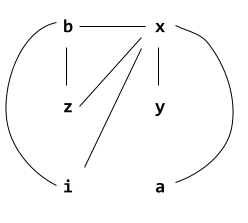
\includegraphics[scale=0.6]{../assets/loc_use1.png}
\end{center}
This is a graph where if there are two variables that had to be live at the same time, then there is an edge. How do we make it so we can have a set of locations where each variable can be assigned to a register that's different from all the things it conflicts with? This problem is known as \textbf{graph coloring}. The idea is that we want to find $k$ colors assigning $1 \hdots k$ to each node such that $k$ is minimal and no edge has the same index for both nodes. A coloring for this graph is 
\begin{center}
    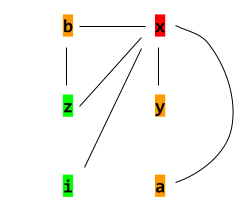
\includegraphics[scale=0.6]{../assets/loc_use2.png}
\end{center}
We only need 3 colors! In terms of what our compiler would output, we would end up with the environment 
\begin{verbatim}
    {x: 1, b: 2, y: 2, a: 2, z: 3, i: 3}\end{verbatim}
In other words, \code{x} gets abstract location 1, \code{b} gets abstract location 2, and so on. Note that this makes a few assumptions: 
\begin{itemize}
    \item All intermediates are carefully named and used (no useless temporaries).
    \item Assuming all temporaries are explicit, this could replace \code{depth(e)}. Note that this means \emph{simple constants!}
    \item All variables are distictly named (although we can rename all non-distinct names if needed).
\end{itemize}

\subsubsection{Algorithm}
The algorithm for this process is as follows: 
\begin{itemize}
    \item Visit last, or innermost, expression first. THis means recurse, then working with result. 
    \item Track set of variables we have seen used, then remove from set at the let-bindings.
\end{itemize}
So, going back to the example code, we have the following set of active variables.
\begin{verbatim}
    (let (b 4)                                  ; {}
        (let (x 10)                             ; {b}
            (let (i (if input                   ; {b, x}
                        (let (z 11) (+ z b))    ; {z, b, x}
                        (let (y 9) (+ y 1))))   ; {y, x}
                (let (a (+ i 5))                ; {i, x}
                    (+ a x)))))                 ; {a, x}\end{verbatim}
For each pair of active variables that appear at the same time, we draw an edge between them in the graph.

\end{document}